\documentclass[../main]{subfiles}
\ifSubfilesClassLoaded{\setcounter{chapter}{2}}{}
\begin{document}

\chapter{Matematika Kriptografi}

\begin{subcpmk}
  \item Sub-CPMK 2.1: Menghitung operasi aritmetika modular dan mengimplementasikan algoritma Euclid diperluas dalam C
  \item Sub-CPMK 2.2: Menentukan bilangan prima, uji primalitas, dan menghitung pangkat modular (fast exponentiation) dalam C
\end{subcpmk}

% ============================================================
% MATERI POKOK
% ============================================================
\section{Aritmetika Modular}

\subsection{Definisi Kongruensi}

Dua bilangan bulat $a$ dan $b$ dikatakan \textbf{kongruen modulo $n$} jika $n$ membagi $(a - b)$. Ditulis:
\[
a \equiv b \pmod{n} \quad \Leftrightarrow \quad n \mid (a - b)
\]

\begin{contoh}
$17 \equiv 2 \pmod{5}$ karena $17 - 2 = 15$ habis dibagi 5. Dengan kata lain, $17 \bmod 5 = 2$.
\end{contoh}

Aritmetika modular membentuk fondasi matematis untuk banyak algoritma kriptografi modern, terutama RSA yang secara fundamental bergantung pada sifat-sifat operasi modulo. Menurut blog 3010tangents, aritmetika modular memungkinkan pasangan tak terhingga dari bilangan untuk memenuhi kendala tertentu, tetapi tidak memungkinkan pengguna untuk mendekripsi pesan tanpa kunci yang tepat. Sifat ini membuat aritmetika modular sangat ideal untuk kriptografi karena menciptakan masalah satu arah (one-way problem) yang mudah dihitung dalam satu arah tetapi sangat sulit dibalik tanpa informasi tambahan.

Analogi jam sering digunakan untuk menjelaskan konsep modular arithmetic di mana jam analog dengan 12 jam secara alami menggunakan operasi modulo 12. Jika jam menunjukkan pukul 11 dan kita ingin mengetahui waktu setelah 4 jam, hasilnya adalah pukul 3, bukan pukul 15, karena dalam sistem 12-jam kita "melilit kembali" setelah mencapai 12. Konsep melilit kembali (wrap-around) ini adalah esensi dari aritmetika modular dan sangat penting dalam kriptografi di mana kita ingin membatasi hasil operasi dalam rentang tertentu.

\subsection{Representasi \texorpdfstring{$\mathbb{Z}_n$}{Z\_n} dan Bilangan Negatif}

Hasil operasi modulo $n$ direpresentasikan sebagai kelas sisa dalam himpunan $\mathbb{Z}_n$ \cite{shoup2009,stanford_numbertheory}. Secara eksplisit, $\mathbb{Z}_n = \{0, 1, \ldots, n-1\}$. Dalam implementasi, nilai negatif sering dinormalisasi dengan:
\[
a \bmod n = ((a \bmod n) + n) \bmod n
\]
sehingga hasil selalu berada di rentang $0$ sampai $n-1$.

\begin{contoh}
$-3 \bmod 11 = 8$ karena $-3 \equiv 8 \pmod{11}$.
\end{contoh}

\begin{figure}[htbp]
  \centering
  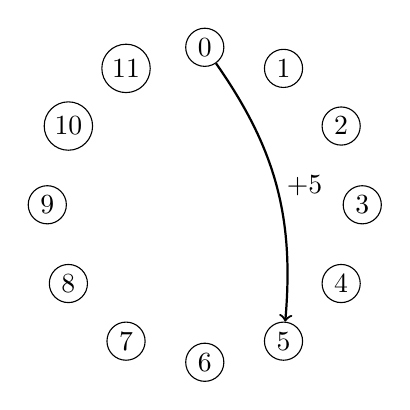
\begin{tikzpicture}[scale=1]
    \foreach \i in {0,...,11} {
      \node[circle, draw, inner sep=2pt] (n\i) at ({90-30*\i}:2) {\i};
    }
    \draw[->, thick] (n0) to[bend left=20] node[midway, right] {$+5$} (n5);
  \end{tikzpicture}
  \caption{Representasi jam aritmetika modular (mod 12).}
\end{figure}

Dalam implementasi kriptografi, representasi $\mathbb{Z}_n$ sangat penting untuk memastikan konsistensi hasil operasi dan mencegah error yang disebabkan oleh nilai negatif atau overflow. Normalisasi nilai negatif dengan menambahkan modulus sebelum mengambil modulo lagi memastikan bahwa semua hasil berada dalam rentang yang diharapkan. Pendekatan ini sangat penting dalam implementasi algoritma RSA di mana operasi modular dilakukan berulang kali pada bilangan yang sangat besar.

\subsection{Operasi Dasar}

Aritmetika modular memenuhi sifat-sifat \cite{trappe2006}:
\begin{itemize}
  \item $(a + b) \bmod n = ((a \bmod n) + (b \bmod n)) \bmod n$
  \item $(a - b) \bmod n = ((a \bmod n) - (b \bmod n) + n) \bmod n$
  \item $(a \cdot b) \bmod n = ((a \bmod n) \cdot (b \bmod n)) \bmod n$
\end{itemize}

\begin{contoh}
$(8 - 13) \bmod 11 = (-5) \bmod 11 = 6$.
\end{contoh}

Sifat distributif aritmetika modular memungkinkan optimasi komputasi yang signifikan dalam implementasi kriptografi, terutama saat bekerja dengan bilangan yang sangat besar seperti dalam RSA. Dengan mengurangi setiap operan terlebih dahulu sebelum melakukan operasi aritmetika, kita dapat mencegah overflow dan meningkatkan efisiensi perhitungan. Teknik ini sangat penting dalam implementasi praktis di mana kita harus melakukan operasi modular berulang kali tanpa kehilangan presisi atau performa.

\subsection{Invers Modular}

Jika $a \cdot x \equiv 1 \pmod{n}$, maka $x$ adalah \textbf{invers modular} dari $a$ modulo $n$, ditulis $x = a^{-1} \pmod{n}$.

\begin{konsep}
Invers modular dari $a$ modulo $n$ hanya ada jika $\gcd(a, n) = 1$. Jika $\gcd(a, n) \neq 1$, maka $a$ tidak memiliki invers modulo $n$.
\end{konsep}

\begin{contoh}
$3^{-1} \equiv 7 \pmod{10}$ karena $3 \cdot 7 = 21 \equiv 1 \pmod{10}$.
\end{contoh}

\begin{table}[htbp]
  \centering
  \small
  \begin{tabular}{cc}
    \toprule
    $a$ & $a^{-1} \bmod 11$ \\
    \midrule
    1 & 1 \\
    2 & 6 \\
    3 & 4 \\
    4 & 3 \\
    5 & 9 \\
    6 & 2 \\
    7 & 8 \\
    8 & 7 \\
    9 & 5 \\
    10 & 10 \\
    \bottomrule
  \end{tabular}
  \caption{Invers modular untuk modulus 11.}
\end{table}

Invers modular merupakan konsep fundamental dalam kriptografi kunci publik, terutama dalam algoritma RSA di mana kunci privat dan publik harus saling invers modulo $\phi(n)$. Menurut Sookocheff, Extended Euclidean Algorithm menyediakan metode efisien untuk menghitung invers modular tanpa harus melakukan pencarian brute force yang tidak praktis untuk bilangan besar. Kemampuan menghitung invers modular dengan cepat dan akurat sangat penting untuk generasi kunci RSA yang aman dan efisien.

\subsection{Pembagian Modular}

Pembagian modular didefinisikan melalui invers: 
\[
\frac{a}{b} \bmod n \equiv a \cdot b^{-1} \bmod n
\]
dengan syarat $\gcd(b, n) = 1$ \cite{rosulek2021}. Jika syarat tidak terpenuhi, pembagian modular tidak terdefinisi.

\begin{contoh}
$4 / 3 \bmod 11 = 4 \cdot 4 \bmod 11 = 5$, karena $3^{-1} \equiv 4 \pmod{11}$.
Sebaliknya, $2 / 6 \bmod 10$ tidak terdefinisi karena $\gcd(6, 10) = 2$.
\end{contoh}

Pembagian modular sangat penting dalam protokol kriptografi modern seperti Diffie-Hellman key exchange dan skema tanda tangan digital. Dalam implementasi praktis, pembagian modular harus dilakukan dengan hati-hati untuk memastikan bahwa pembagi memiliki invers modular sebelum melakukan operasi. Kegagalan memeriksa syarat $\gcd(b, n) = 1$ dapat menyebabkan error runtime atau hasil yang tidak diharapkan dalam aplikasi kriptografi.

\section{Pembagi Persekutuan Terbesar (PBB) dan Algoritma Euclidean}

Dalam kriptografi, kita sering perlu mengetahui apakah dua bilangan memiliki pembagi yang sama atau apakah sebuah bilangan memiliki invers modulo. Alat utama untuk melakukan hal ini adalah konsep \textbf{Pembagi Persekutuan Terbesar} (\textit{Greatest Common Divisor} atau GCD).

\subsection{Definisi PBB}

PBB dari dua bilangan bulat $a$ dan $b$ (tidak keduanya nol) adalah bilangan bulat positif terbesar yang membagi habis $a$ dan juga membagi habis $b$. Notasi yang digunakan adalah $\text{PBB}(a, b)$ atau $\gcd(a, b)$.

\textbf{Contoh}:
Pembagi dari 12 adalah $\{1, 2, 3, 4, 6, 12\}$.
Pembagi dari 18 adalah $\{1, 2, 3, 6, 9, 18\}$.
Pembagi persekutuan dari 12 dan 18 adalah $\{1, 2, 3, 6\}$.
Maka, $\text{PBB}(12, 18) = 6$.

\subsection{Bilangan Relatif Prima (\textit{Coprime})}

Dua bilangan bulat $a$ dan $b$ dikatakan \textbf{relatif prima} atau \textbf{coprime} jika pembagi persekutuan terbesar dari keduanya adalah 1:
\[ \text{PBB}(a, b) = 1 \]
Konsep ini sangat krusial dalam kriptografi. Sebagai contoh, dalam Affine Cipher, kunci perkalian $a$ harus relatif prima dengan modulus $n=26$. Jika $\text{PBB}(a, 26) \neq 1$, maka beberapa huruf plainteks akan menghasilkan cipherteks yang sama, sehingga pesan tidak dapat didekripsi secara unik.

\subsection{Algoritma Euclidean}

Untuk bilangan yang sangat besar, mencari PBB dengan mendaftar semua pembagi tidaklah efisien. Algoritma Euclidean menyediakan metode yang jauh lebih cepat berdasarkan prinsip bahwa PBB dari dua bilangan tidak berubah jika bilangan yang lebih besar digantikan oleh sisa baginya terhadap bilangan yang lebih kecil.

\textbf{Prinsip Dasar}:
\[ \text{PBB}(a, b) = \text{PBB}(b, a \pmod{b}) \]

\textbf{Langkah-langkah Algoritma Euclidean}:
\begin{enumerate}
    \item Misalkan kita ingin mencari $\text{PBB}(a, b)$ dengan $a > b$.
    \item Bagi $a$ dengan $b$ untuk mendapatkan sisa $r$: $a = qb + r$.
    \item Jika $r = 0$, maka $\text{PBB}(a, b) = b$.
    \item Jika $r \neq 0$, maka ulangi proses dengan mengganti $a$ menjadi $b$, dan $b$ menjadi $r$.
\end{enumerate}

\textbf{Contoh Numerik}: Hitung $\text{PBB}(252, 105)$.
\begin{align*}
    252 &= 2 \cdot 105 + 42 \quad \rightarrow \text{PBB}(252, 105) = \text{PBB}(105, 42) \\
    105 &= 2 \cdot 42 + 21 \quad \rightarrow \text{PBB}(105, 42) = \text{PBB}(42, 21) \\
    42 &= 2 \cdot 21 + 0 \quad \rightarrow \text{Selesai!}
\end{align*}
Maka, $\text{PBB}(252, 105) = 21$.

\subsection{Efisiensi Komputasi}

Kekuatan Algoritma Euclidean terletak pada kecepatannya. Secara matematis, jumlah langkah yang dibutuhkan untuk menemukan PBB tidak akan pernah melebihi lima kali jumlah digit dari bilangan yang lebih kecil (Teorema Lamé). Dalam notasi kompleksitas, algoritma ini berjalan dalam waktu $O(\log(\min(a, b)))$, yang membuatnya sangat efisien bahkan untuk angka dengan ribuan digit yang digunakan dalam standar keamanan modern.

\section{Teori Bilangan: Prima dan Fermat--Euler}

\subsection{Bilangan Prima}

Bilangan prima adalah bilangan bulat $p > 1$ yang hanya habis dibagi oleh 1 dan dirinya sendiri. Bilangan prima penting dalam kriptografi karena menjadi dasar pembangkitan kunci RSA \cite{shoup2009}.

Bilangan prima membentuk fondasi keamanan dalam banyak algoritma kriptografi modern \cite{stallings2017}. RSA bergantung pada kesulitan faktorisasi: mengalikan dua bilangan prima besar mudah, tetapi memfaktorkan hasilnya kembali sangat sulit secara komputasional.

Dalam praktik, RSA dan Diffie-Hellman menggunakan bilangan prima yang sangat besar (ratusan atau ribuan digit) untuk memastikan keamanan. Generasi bilangan prima ini memerlukan algoritma uji primalitas yang efisien seperti Miller-Rabin yang dapat memverifikasi primalitas dengan probabilitas tinggi tanpa harus melakukan faktorisasi penuh. Ketersediaan bilangan prima yang aman dan acak sangat penting untuk keamanan jangka panjang sistem kriptografi kunci publik.

\subsection{Uji Primalitas}

\textbf{Uji pembagian (trial division)}: Cek apakah $n$ habis dibagi oleh bilangan prima $\leq \sqrt{n}$. Metode ini sederhana tetapi lambat untuk bilangan besar.

\textbf{Sieve of Eratosthenes}: Membangun daftar prima hingga batas $N$ dengan mencoret kelipatan bilangan. Cocok untuk menghasilkan daftar prima kecil-menengah \cite{stein2008}.

\textbf{Miller-Rabin}: Uji probabilistik yang sangat cepat untuk bilangan besar. Dengan beberapa basis acak, peluang salah (bilangan komposit terdeteksi sebagai prima) menjadi sangat kecil \cite{shoup2009}.

\begin{table}[htbp]
  \centering
  \small
  \begin{tabular}{>{\raggedright\arraybackslash}p{3.5cm}>{\raggedright\arraybackslash}p{4.5cm}>{\raggedright\arraybackslash}p{4.5cm}}
    \toprule
    Metode & Ide Utama & Kegunaan \\
    \midrule
    Trial division & Bagi hingga $\sqrt{n}$ & Bilangan kecil, verifikasi sederhana \\
    Sieve of Eratosthenes & Eliminasi kelipatan & Daftar prima sampai batas $N$ \\
    Miller-Rabin & Uji probabilistik modular & Bilangan besar (RSA) \\
    \bottomrule
  \end{tabular}
  \caption{Perbandingan ringkas uji primalitas.}
\end{table}

Uji primalitas probabilistik seperti Miller-Rabin sangat penting untuk protokol kriptografi \cite{shoup2009}. Algoritma ini cepat dan memverifikasi primalitas dengan probabilitas kesalahan yang dapat diabaikan, ideal untuk generasi bilangan prima besar dalam RSA.

Pemilihan metode uji primalitas tergantung pada ukuran bilangan dan kebutuhan aplikasi. Untuk bilangan kecil, trial division atau sieve of Eratosthenes mungkin sudah cukup, tetapi untuk bilangan besar yang digunakan dalam kriptografi modern, Miller-Rabin atau uji primalitas probabilistik lainnya menjadi satu-satunya pilihan praktis. Trade-off antara kecepatan dan kepastian menjadi pertimbangan penting dalam desain sistem kriptografi.

\subsection{Teorema Fermat Kecil dan Bilangan Carmichael}

\textbf{Teorema Fermat Kecil}: Jika $p$ prima dan $\gcd(a, p) = 1$, maka:
\[
a^{p-1} \equiv 1 \pmod{p}
\]

\textbf{Catatan penting}: Ada bilangan komposit yang lolos uji Fermat untuk banyak basis $a$, disebut bilangan Carmichael. Contoh klasik adalah $561 = 3 \cdot 11 \cdot 17$ \cite{rosulek2021}.

Teorema Fermat Kecil menyediakan dasar matematis untuk banyak protokol kriptografi dan algoritma uji primalitas. Dalam konteks keamanan, bilangan Carmichael menimbulkan tantangan khusus karena dapat menipu uji primalitas sederhana yang hanya mengandalkan Teorema Fermat Kecil. Keberadaan bilangan-bilangan ini menunjukkan mengapa uji primalitas yang lebih canggih seperti Miller-Rabin diperlukan untuk aplikasi kriptografi yang andal.

Pemahaman tentang bilangan Carmichael sangat penting dalam desain sistem kriptografi karena mereka merupakan contoh counter-intuitif di mana sifat yang berlaku untuk bilangan prima juga berlaku untuk beberapa bilangan komposit. Pengetahuan ini membantu kriptografer untuk menghindari kelemahan dalam implementasi uji primalitas dan memastikan bahwa hanya bilangan prima sejati yang digunakan dalam generasi kunci.

\subsection{Fungsi Euler \texorpdfstring{$\varphi(n)$}{phi(n)}}

\textbf{Fungsi Euler $\varphi(n)$}: Banyaknya bilangan bulat $1 \leq k \leq n$ yang relatif prima dengan $n$. Untuk $n$ dengan faktorisasi prima:
\[
\varphi(n) = n \prod_{p \mid n} \left(1 - \frac{1}{p}\right)
\]
Khusus untuk $n = p^k$, berlaku $\varphi(p^k) = p^k - p^{k-1}$ \cite{stanford_numbertheory}.

Untuk $n = p \cdot q$ dengan $p, q$ prima: $\varphi(n) = (p-1)(q-1)$.

\begin{table}[htbp]
  \centering
  \small
  \begin{tabular}{cc}
    \toprule
    $n$ & $\varphi(n)$ \\
    \midrule
    1 & 1 \\
    2 & 1 \\
    3 & 2 \\
    4 & 2 \\
    5 & 4 \\
    6 & 2 \\
    7 & 6 \\
    8 & 4 \\
    9 & 6 \\
    10 & 4 \\
    \bottomrule
  \end{tabular}
  \caption{Nilai $\varphi(n)$ untuk $n=1$ sampai $10$.}
\end{table}

Fungsi Euler Totient $\varphi(n)$ sangat fundamental dalam kriptografi kunci publik, terutama RSA, di mana ia menentukan ukuran grup perkalian modular dan jumlah kunci privat yang mungkin. Menurut sifat $\varphi(n) = (p-1)(q-1)$ untuk $n = p \cdot q$, kita dapat melihat bagaimana pengetahuan tentang faktorisasi $n$ langsung memberikan informasi tentang $\varphi(n)$. Ini adalah alasan mengapa keamanan RSA bergantung pada kesulitan memfaktorkan $n$.

Dalam implementasi RSA, $\varphi(n)$ digunakan untuk menghitung invers modular dari eksponen publik untuk mendapatkan kunci privat. Hubungan antara $\varphi(n)$ dan keamanan RSA sangat erat: jika penyerang dapat menghitung $\varphi(n)$, mereka dapat dengan mudah memecahkan sistem. Oleh karena itu, keamanan RSA secara langsung terkait dengan kesulitan menghitung $\varphi(n)$ tanpa mengetahui faktorisasi prima dari $n$.

\subsection{Teorema Euler}

Jika $\gcd(a, n) = 1$, maka:
\[
a^{\varphi(n)} \equiv 1 \pmod{n}
\]

Teorema Euler menjadi dasar matematis untuk RSA: $a^{k \cdot \varphi(n) + 1} \equiv a \pmod{n}$.

Teorema Euler menggeneralisasi Teorema Fermat Kecil dan membentuk landasan matematis untuk operasi kriptografi kunci publik. Dalam RSA, teorema ini menjamin bahwa $m^{e \cdot d} \equiv m \pmod{n}$ ketika $e \cdot d \equiv 1 \pmod{\varphi(n)}$, yang merupakan prinsip dasar enkripsi dan dekripsi RSA. Sifat ini memastikan bahwa operasi dekripsi benar-benar membalikkan operasi enkripsi ketika kunci yang tepat digunakan.

Penting untuk dicatat bahwa Teorema Euler hanya berlaku ketika $\gcd(a, n) = 1$, yang dalam konteks RSA berarti bahwa pesan harus relatif prima dengan modulus. Dalam praktik, ini biasanya tidak menjadi masalah karena modulus $n$ adalah produk dari dua bilangan prima besar dan pesan umumnya jauh lebih kecil dari $n$, membuat probabilitas bahwa $\gcd(m, n) \neq 1$ sangat kecil. Namun, implementasi yang robust harus memeriksa kondisi ini untuk memastikan operasi dekripsi bekerja dengan benar.

\subsection{Chinese Remainder Theorem}

\textbf{Chinese Remainder Theorem (CRT)}: Jika $n_1,\ldots,n_k$ saling koprima dan $a_1,\ldots,a_k$ sebarang bilangan bulat, maka terdapat tepat satu solusi $x$ modulo $N = n_1 \cdots n_k$ untuk sistem kongruensi:
\[
x \equiv a_i \pmod{n_i} \quad \text{untuk } i = 1,\ldots,k
\]

CRT memungkinkan komputasi modulo $N$ dilakukan secara paralel dalam modulus yang lebih kecil, mempercepat operasi seperti dekripsi RSA \cite{stallings2017}. Dalam implementasi RSA, CRT dipakai untuk menghitung $m = c^d \bmod n$ via $m_p = c^d \bmod p$ dan $m_q = c^d \bmod q$, lalu menggabungkan hasil dengan CRT.

\section{Bilangan Prima dan Pengujian Primalitas}

Bilangan prima adalah batu bata penyusun seluruh sistem kriptografi modern. Keamanan algoritma seperti RSA tidak didasarkan pada kerahasiaan algoritma, tetapi pada fakta matematis bahwa mengalikan dua bilangan prima besar sangatlah mudah, sementara memfaktorkan hasil kalinya kembali menjadi dua prima asal adalah masalah yang sangat sulit secara komputasi.

\subsection{Definisi dan Sifat Bilangan Prima}

Bilangan prima adalah bilangan bulat positif yang lebih besar dari 1 dan hanya memiliki dua pembagi positif: 1 dan dirinya sendiri. Bilangan bulat positif yang lebih besar dari 1 dan bukan prima disebut sebagai bilangan komposit.

Kriptografi menggunakan bilangan prima yang sangat besar, seringkali mencapai ribuan bit. Menghasilkan bilangan prima besar membutuhkan proses yang efisien karena kita tidak bisa menggunakan metode pembagian biasa (\textit{Trial Division}) yang akan memakan waktu jutaan tahun untuk angka sebesar itu.

\subsection{Algoritma Pengujian Primalitas}

Untuk menemukan bilangan prima besar, kita tidak mencari bilangan prima, tetapi memilih angka acak besar dan kemudian \textbf{mengujinya} apakah angka tersebut prima.

\begin{enumerate}
    \item \textbf{Sieve of Eratosthenes}: Metode klasik untuk menemukan semua bilangan prima dalam rentang tertentu. Namun, metode ini tidak efisien untuk angka yang sangat besar karena membutuhkan memori yang masif.
    \item \textbf{Pengujian Probabilistik (Miller-Rabin Test)}: Sebagian besar sistem kriptografi menggunakan pengujian probabilistik. Algoritma Miller-Rabin tidak memberikan kepastian 100\%, tetapi dapat memberikan jaminan bahwa suatu bilangan adalah "kemungkinan besar prima" (\textit{probably prime}) dengan tingkat kesalahan yang sangat kecil (misalnya $2^{-100}$). Jika suatu bilangan gagal dalam satu putaran uji Miller-Rabin, maka ia pasti komposit. Jika lolos, ia kemungkinan besar prima.
\end{enumerate}

\subsection{Pentingnya Bilangan Prima dalam Kriptografi}

Penggunaan bilangan prima bukan tanpa alasan. Sifat-sifatnya memberikan jaminan keamanan:
\begin{itemize}
    \item \textbf{Asimetri Komputasi}: Perbedaan kecepatan antara perkalian (mudah) dan faktorisasi (sulit) menciptakan "pintu satu arah" (\textit{trapdoor function}) yang menjadi dasar RSA.
    \item \textbf{Struktur Grup}: Bilangan prima $p$ memastikan bahwa himpunan $\{1, 2, \dots, p-1\}$ membentuk grup multiplikatif modulo $p$, yang menjamin bahwa setiap elemen memiliki invers modulo.
\end{itemize}

\begin{catatan}
Dalam implementasi nyata, bilangan prima yang digunakan untuk RSA harus dipilih secara acak dan sangat besar agar terhindar dari serangan faktorisasi menggunakan algoritma seperti \textit{General Number Field Sieve} (GNFS).
\end{catatan}

\section{Teori Informasi dan Entropi}

\subsection{Apa Itu Teori Informasi?}

\textbf{Teori informasi} (\textit{information theory}) adalah cabang ilmu yang mempelajari kuantisasi, penyimpanan, transmisi, dan pengolahan informasi \cite{munir_slides_itb,shannon1948}. Dua contoh sederhana:
\begin{itemize}
  \item \textbf{Kuantisasi}: 1 bit cukup untuk mengodekan jenis kelamin (M/F), 3 bit untuk nama hari (7 hari), dan 4 bit untuk digit 0 sampai 9.
  \item \textbf{Penyimpanan}: pemampatan (kompresi) data mengurangi ukuran ruang simpan dengan membuang redundansi.
\end{itemize}

Claude Shannon meletakkan dasar teori ini dalam ``A Mathematical Theory of Communication'' (1948), lalu menerapkannya pada kriptografi dalam ``Communication Theory of Secrecy Systems'' (1949) \cite{shannon1948,shannon1949}.

\subsection{Entropi}

Metrik terpenting dalam teori informasi adalah \textbf{entropi}, yang mengukur ketidakpastian atau jumlah rata-rata informasi dalam pesan, biasanya dinyatakan dalam bit \cite{munir_slides_itb,entropy_wikipedia}. Semakin acak suatu data, semakin tinggi entropinya; ciphertext yang baik adalah pesan dengan entropi tinggi.

\begin{konsep}
Entropi pesan $X$ yang terdiri atas $n$ simbol berbeda $x_1, \ldots, x_n$ dengan peluang kemunculan $p(x_i)$:
\[
H(X) = -\sum_{i=1}^{n} p(x_i) \log_2 p(x_i) \quad \text{(bit per simbol)}
\]
\end{konsep}

\begin{contoh}
Misalkan $X = \texttt{AABBCBDB}$ (8 karakter). Ada $n = 4$ simbol berbeda dengan peluang $p(A) = 2/8$, $p(B) = 4/8$, $p(C) = 1/8$, $p(D) = 1/8$ \cite{munir_slides_itb}. Maka:
\begin{align*}
H(X) &= -\left[\tfrac{1}{4}\log_2\tfrac{1}{4} + \tfrac{1}{2}\log_2\tfrac{1}{2} + \tfrac{1}{8}\log_2\tfrac{1}{8} + \tfrac{1}{8}\log_2\tfrac{1}{8}\right] \\
&= -\left[\tfrac{1}{4}(-2) + \tfrac{1}{2}(-1) + \tfrac{1}{8}(-3) + \tfrac{1}{8}(-3)\right] \\
&= \tfrac{1}{2} + \tfrac{1}{2} + \tfrac{3}{8} + \tfrac{3}{8} = 1{,}75 \text{ bit per simbol.}
\end{align*}
\end{contoh}

\subsection{Batas Nilai Entropi}

Nilai entropi selalu berada dalam rentang
\[
0 \le H(X) \le \log_2 n.
\]
\begin{itemize}
  \item \textbf{Minimum} ($H = 0$): tidak ada ketidakpastian, terjadi jika hanya ada satu simbol dengan peluang 1. Contoh: pesan hanya berisi huruf A, sehingga $H = -1 \cdot \log_2 1 = 0$.
  \item \textbf{Maksimum} ($H = \log_2 n$): terjadi jika semua simbol berpeluang sama, yaitu $1/n$; setiap simbol membawa informasi maksimal. Contoh: empat simbol berpeluang $0{,}25$ memberi $H = \log_2 4 = 2$ bit.
\end{itemize}

Untuk teks yang hanya memakai 26 huruf alfabet (A--Z), entropi maksimum terjadi jika setiap huruf berpeluang $1/26$:
\[
H_{\max} = -\sum_{i=1}^{26} \tfrac{1}{26}\log_2\tfrac{1}{26} = \log_2 26 \approx 4{,}7004 \text{ bit/karakter.}
\]

\begin{table}[htbp]
\centering
\small
\begin{tabular}{|l|c|c|}
\toprule
\textbf{Alfabet} & \textbf{Jumlah Simbol} & $H_{\max}$ (bit/simbol) \\
\midrule
Biner & 2 & 1 \\
Desimal & 10 & $\approx 3{,}32$ \\
Huruf A--Z & 26 & $\approx 4{,}70$ \\
ASCII cetak (\textit{printable}) & 95 & $\approx 6{,}57$ \\
ASCII 8-bit & 256 & 8 \\
\bottomrule
\end{tabular}
\caption{Entropi maksimum untuk beberapa alfabet.}
\end{table}

\subsection{Entropi Plaintext dan Ciphertext}

Makin besar entropi ciphertext, makin sulit ciphertext dipecahkan, karena pola bahasa pada plaintext tidak lagi terlihat. Hal yang sama tampak secara visual pada cipher-image di Bab~II (Gambar~\ref{fig:plain-cipher-image}): citra terenkripsi menyerupai derau acak, yaitu data berentropi tinggi. Contoh berikut diambil dari slide kuliah \cite{munir_slides_itb}: sebuah paragraf berita berbahasa Indonesia dienkripsi menjadi ciphertext yang hanya memakai huruf A--Z (Gambar~\ref{fig:entropi-ternate}).

\begin{figure}[htbp]
\centering
\fbox{\begin{minipage}[t][4.4cm][t]{0.4\textwidth}
\footnotesize
Dinas Pendidikan Kota Ternate meminta kepada pihak sekolah dan orang tua siswa untuk jenjang pendidikan SD dan SMP se-Kota Ternate untuk melarang para siswa membawa permainan lato-lato yang sedang tren itu ke sekolah, karena akan mengganggu kegiatan belajar mengajar yang dinilai berbahaya sehingga mengantisipasi kecelakaan bagi anak di daerah itu.
\end{minipage}}\hfill
\fbox{\begin{minipage}[t][4.4cm][t]{0.53\textwidth}
\footnotesize\ttfamily
HAWFHZDOHAHANGOMKLGFCVWFLBOCPRKFGHNOFNIN\\
SPGNLHMPFVBEFWMVFWTBWRHSFZRWKFQMVHPAFWIK\\
DOHAHANGPFEWNFPFNKLHMPFGLBAMGFCXKFQMOCFV\\
AVKANIAVHSFZRNCODGAFOHYUVGWGFOFGXEGFMLFWIT\\
HEFWTBVCPAYQOBLHMPFVBPVADOVGNWFGNOVCARKVA\\
RQOBRGGFWHCVFGVYYUDORVGVYCFWABAPVSVGCHGCI\\
DRFIFHBAPVQRVOCKAFWSGSHSNIHSOBDHFVNGFWDGRGRF\\
WGNHANFCVIDGSWZ
\end{minipage}}\\[2pt]
\begin{minipage}{0.42\textwidth}\centering\small (a) Plainteks $P$\end{minipage}\hfill
\begin{minipage}{0.55\textwidth}\centering\small (b) Cipherteks $C$\end{minipage}\\[12pt]
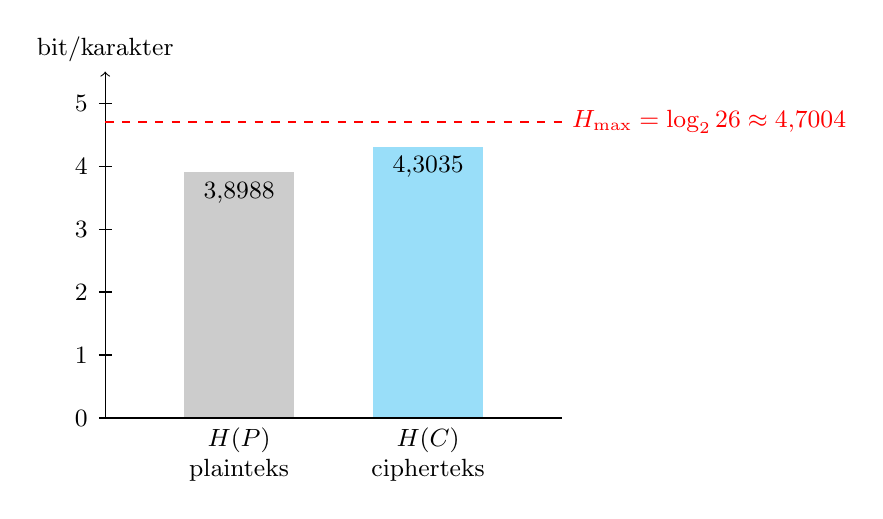
\begin{tikzpicture}[yscale=0.8, font=\small]
  \fill[gray!40] (1.0,0) rectangle (2.4,3.8988);
  \fill[cyan!40] (3.4,0) rectangle (4.8,4.3035);
  \node[below] at (1.7,3.8988) {3,8988};
  \node[below] at (4.1,4.3035) {4,3035};
  \draw[->] (0,0) -- (0,5.5) node[above] {bit/karakter};
  \draw (0,0) -- (5.8,0);
  \foreach \y in {0,...,5} {
    \draw (-0.08,\y) -- (0.08,\y);
    \node[left] at (-0.1,\y) {\y};
  }
  \draw[dashed, red, thick] (0,4.7004) -- (5.8,4.7004) node[right] {$H_{\max} = \log_2 26 \approx 4{,}7004$};
  \node[below, align=center] at (1.7,0) {$H(P)$\\plainteks};
  \node[below, align=center] at (4.1,0) {$H(C)$\\cipherteks};
\end{tikzpicture}\\[2pt]
{\small (c) Entropi plainteks dan cipherteks dibandingkan dengan entropi maksimum}
\caption{Enkripsi menaikkan entropi: cipherteks mencapai sekitar 91,55\% dari entropi maksimum teks 26 huruf \cite{munir_slides_itb}.}
\label{fig:entropi-ternate}
\end{figure}

\begin{contoh}
\begin{itemize}
  \item Entropi plaintext: $H(P) = 3{,}8988$ bit/karakter.
  \item Entropi ciphertext: $H(C) = 4{,}3035$ bit/karakter.
  \item Ciphertext mencapai $\dfrac{4{,}3035}{4{,}7004} \times 100\% \approx 91{,}55\%$ dari entropi maksimum teks 26 huruf.
\end{itemize}
Enkripsi menaikkan entropi: distribusi huruf pada ciphertext menjadi jauh lebih merata dibanding plaintext.
\end{contoh}

\subsection{Laju Bahasa dan Redundansi}

\textbf{Laju bahasa} (\textit{language rate}) adalah entropi per simbol dalam teks nyata suatu bahasa. Bahasa Inggris memiliki laju sekitar 1{,}0--1{,}5 bit/huruf, jauh di bawah $H_{\max} \approx 4{,}7$ bit/huruf \cite{shannon1951}.

\textbf{Redundansi} didefinisikan sebagai:
\[
R = 1 - \frac{H_{\text{aktual}}}{H_{\text{maksimum}}}
\]
Untuk perkiraan $H_{\text{aktual}} \approx 1{,}5$ dan $H_{\max} \approx 4{,}7$: $R \approx 0{,}68$ (sekitar 68\%). Redundansi inilah yang memungkinkan \textit{analisis frekuensi} memecah cipher substitusi monoalfabetik.

\begin{table}[htbp]
\centering
\small
\begin{tabular}{lcc}
\toprule
Sumber & Entropi Maksimum & Entropi Aktual \\
\midrule
Alfabet seragam (26 huruf) & 4{,}7 bit & 4{,}7 bit \\
Bahasa Inggris & 4{,}7 bit & $\approx$1{,}5 bit \\
Biner seragam & 1{,}0 bit & 1{,}0 bit \\
\bottomrule
\end{tabular}
\caption{Perbandingan entropi maksimum vs aktual.}
\end{table}

\begin{figure}[htbp]
\centering
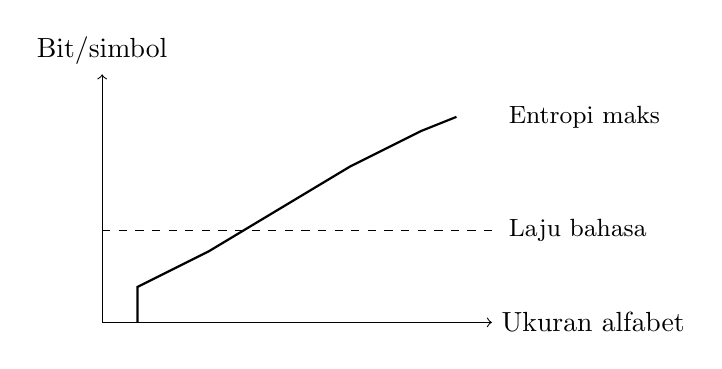
\begin{tikzpicture}[scale=0.9]
  \draw[->] (0,0) -- (5.5,0) node[right] {Ukuran alfabet};
  \draw[->] (0,0) -- (0,3.5) node[above] {Bit/simbol};
  \draw[thick] (0.5,0) -- (0.5,0.5) -- (1.5,1) -- (2.5,1.6) -- (3.5,2.2) -- (4.5,2.7) -- (5,2.9);
  \draw[dashed] (0,1.3) -- (5.5,1.3);
  \node[right, font=\small] at (5.6,2.9) {Entropi maks};
  \node[right, font=\small] at (5.6,1.3) {Laju bahasa};
\end{tikzpicture}
\caption{Ilustrasi: entropi maksimum naik dengan ukuran alfabet; laju bahasa aktual lebih rendah karena redundansi.}
\end{figure}

Cipher yang ideal menghasilkan ciphertext dengan entropi tinggi dan redundansi rendah sehingga penyerang sulit memanfaatkan pola bahasa.

\subsection{Pengayaan: Unicity Distance dan Perfect Secrecy}

\begin{catatan}
Subbagian ini bersifat \textbf{pengayaan} dan bukan prasyarat Sub-CPMK 2.3. Manfaatnya terasa saat membahas kriptanalisis cipher klasik (Bab~IV) dan desain cipher modern (Bab~V).
\end{catatan}

\textbf{Unicity distance} adalah panjang ciphertext minimum di mana hanya ada satu plaintext yang masuk akal yang dapat menghasilkan ciphertext tersebut \cite{shannon1949}. Untuk cipher dengan entropi kunci $H(K)$ dan redundansi per simbol $D$:
\[
U = \frac{H(K)}{D}
\]

\begin{contoh}
Untuk Caesar cipher:
\begin{itemize}
  \item Ruang kunci: 25 kemungkinan; $H(K) = \log_2 25 \approx 4{,}64$ bit
  \item Redundansi bahasa Inggris: $D \approx 4{,}7 - 1{,}5 = 3{,}2$ bit/huruf
  \item $U \approx 4{,}64 / 3{,}2 \approx 1{,}45$ huruf --- secara teoretis hanya perlu sedikit ciphertext untuk memecahkan Caesar secara unik
\end{itemize}
\end{contoh}

\begin{table}[htbp]
\centering
\small
\begin{tabular}{lcc}
\toprule
Cipher & Ukuran Kunci & Unicity Distance \\
\midrule
Caesar (25 kunci) & 4{,}64 bit & $\approx$2 huruf \\
Vigen\`{e}re ($26^k$ kunci) & $k \cdot 4{,}7$ bit & $\approx 1{,}5k$ huruf \\
DES (56-bit) & 56 bit & $\approx$17{,}5 huruf \\
AES-128 & 128 bit & $\approx$40 huruf \\
\bottomrule
\end{tabular}
\caption{Unicity distance untuk berbagai cipher (perkiraan).}
\end{table}

\begin{catatan}
Unicity distance adalah batas teoretis tentang berapa banyak ciphertext yang secara informasi cukup untuk menentukan kunci, bukan ukuran kemudahan serangan. Memecahkan AES tetap tidak layak secara komputasi walaupun unicity distance-nya hanya sekitar 40 huruf.
\end{catatan}

\textbf{Perfect secrecy} terjadi ketika ciphertext tidak memberikan informasi apa pun tentang plaintext. Shannon membuktikan syarat perlunya $H(K) \geq H(P)$. One-Time Pad memenuhinya jika kunci acak sepanjang plaintext dan hanya dipakai sekali. Definisi formal \textit{perfect secrecy}, pembuktiannya untuk OTP, serta alasan OTP tidak praktis dibahas pada subbab One-Time Pad di Bab~IV.

\begin{contoh}
Plaintext 8-bit dan kunci acak 8-bit di-XOR menghasilkan ciphertext; setiap kunci yang mungkin memberi ciphertext berbeda sehingga ciphertext saja tidak mengungkap plaintext.
\end{contoh}

Implikasi untuk desain cipher:
\begin{enumerate}
  \item \textbf{Kerentanan analisis frekuensi}: redundansi bahasa alami membuat cipher substitusi rentan.
  \item \textbf{Kebutuhan ruang kunci yang besar}: kunci pendek mudah dicari secara menyeluruh (\textit{brute force}).
  \item \textbf{Confusion dan diffusion} (Shannon): \textit{confusion} menyembunyikan hubungan antara kunci dan ciphertext; \textit{diffusion} menyebar pengaruh satu bit plaintext ke banyak bit ciphertext.
\end{enumerate}

\subsection{Koneksi ke Bab-Bab Berikutnya}

\begin{itemize}
  \item \textbf{Bab IV}: analisis frekuensi pada cipher klasik memanfaatkan redundansi bahasa
  \item \textbf{Bab V}: desain cipher modern menekankan confusion dan diffusion
  \item \textbf{Bab VI}: pemilihan ukuran kunci berkaitan dengan ruang kunci
\end{itemize}


% ============================================================
% AKTIVITAS PEMBELAJARAN
% ============================================================

\begin{aktivitas}
  \item \textbf{Praktikum C}: Implementasikan fungsi \code{extended\_gcd} dan \code{mod\_inverse}. Uji dengan berbagai pasangan $(a, m)$.
  
  \item \textbf{Praktikum C}: Implementasikan \code{mod\_pow} untuk fast exponentiation. Bandingkan waktu eksekusi dengan pendekatan naif untuk $a^{1000000} \bmod n$.
  
  \item \textbf{Latihan Numerik}: Hitung secara manual: $17^{-1} \pmod{26}$, $5^{100} \bmod 13$.
  
  \item \textbf{Algoritma}: Jelaskan mengapa invers modular hanya ada jika $\gcd(a, n) = 1$. Berikan contoh bilangan yang tidak memiliki invers modulo 10.
\end{aktivitas}

% ============================================================
% LATIHAN DAN REFLEKSI
% ============================================================

\begin{latihan}
  \item Hitung: $ (23 + 47) \bmod 11 $, $ (23 \cdot 47) \bmod 11 $.
  
  \item Tentukan invers modular dari 7 modulo 26. Gunakan algoritma Euclid diperluas.
  
  \item Jelaskan teorema Fermat kecil dan teorema Euler. Kapan masing-masing berlaku?
  
  \item Hitung $3^{644} \bmod 645$ menggunakan fast exponentiation.
  
  \item Implementasikan dalam C: fungsi yang mengecek apakah $n$ relatif prima dengan $m$ (yaitu $\gcd(n, m) = 1$).
  
  \item \textbf{Refleksi}: Bagaimana keterkaitan matematika kriptografi (modular, Euclid, Fermat) dengan algoritma RSA?
\end{latihan}

% ============================================================
% ASESMEN
% ============================================================

\begin{asesmen}
\textbf{Instrumen Penilaian untuk Sub-CPMK 2.1, 2.2}

\textbf{A. Pilihan Ganda}

\begin{enumerate}
  \item Invers modular dari $a$ modulo $n$ hanya ada jika:
  \begin{enumerate}
    \item $a > n$
    \item $\gcd(a, n) = 1$
    \item $a$ prima
    \item $n$ prima
  \end{enumerate}
  
  \item Algoritma fast exponentiation untuk menghitung $a^b \bmod n$ memiliki kompleksitas waktu:
  \begin{enumerate}
    \item $O(b)$
    \item $O(\log b)$
    \item $O(n)$
    \item $O(a)$
  \end{enumerate}
  
  \item Untuk $n = p \cdot q$ dengan $p, q$ prima, $\varphi(n)$ sama dengan:
  \begin{enumerate}
    \item $p + q$
    \item $p \cdot q$
    \item $(p-1)(q-1)$
    \item $p - q$
  \end{enumerate}
\end{enumerate}

\textbf{B. Essay dan Coding}

\begin{enumerate}
  \item Jelaskan algoritma Euclid diperluas dan kegunaannya dalam kriptografi.
  
  \item Implementasikan dalam C: \code{mod\_inverse(a, m)} yang mengembalikan $-1$ jika invers tidak ada.
\end{enumerate}

\textbf{Rubrik Penilaian}: Lihat Lampiran A
\end{asesmen}

% ============================================================
% CHECKLIST KOMPETENSI
% ============================================================

\begin{checklist}
  \item Saya dapat melakukan operasi aritmetika modular (penjumlahan, perkalian, invers)
  \item Saya dapat mengimplementasikan algoritma Euclid diperluas dalam C
  \item Saya dapat mengimplementasikan mod inverse dalam C
  \item Saya memahami teorema Fermat dan Euler
  \item Saya dapat mengimplementasikan fast modular exponentiation dalam C
  \item Saya memahami peran matematika kriptografi dalam algoritma RSA
\end{checklist}

% ============================================================
% RANGKUMAN
% ============================================================

\begin{rangkuman}
Bab ini membahas fondasi matematika kriptografi: aritmetika modular, algoritma Euclid dan Euclid diperluas, teori bilangan (prima, teorema Fermat dan Euler), serta fast modular exponentiation. Semua konsep ini menjadi dasar untuk memahami dan mengimplementasikan RSA.

\textbf{Poin Kunci:}
\begin{itemize}
  \item Kongruensi modular: $a \equiv b \pmod{n}$ jika $n \mid (a-b)$
  \item Invers modular hanya ada jika $\gcd(a, n) = 1$
  \item Euclid diperluas: menghitung $\gcd$ sekaligus koefisien Bézout
  \item Fast exponentiation: $O(\log b)$ untuk menghitung $a^b \bmod n$
  \item $\varphi(n) = (p-1)(q-1)$ untuk $n = pq$
\end{itemize}

\textbf{Kata Kunci}: \crypt{Aritmetika Modular}, \crypt{Kongruensi}, \crypt{Algoritma Euclid}, \crypt{Invers Modular}, \crypt{Fast Exponentiation}, \crypt{Fungsi Euler}
\end{rangkuman}

\ifSubfilesClassLoaded{
  \renewcommand{\bibname}{Daftar Pustaka}
  \bibliographystyle{plain}
  \bibliography{../references}
}{}
\end{document}
